%---------------------------------------------------------------------------------
\chapter{NOMA-aided UAV Communications over Bivariate Rician Shadowed Fading Channels}
\label{chap:NOMA_bivariate_Rician_Shadowed}
%---------------------------------------------------------------------------------
\section{Introduction}

As one of the key enabling technologies being considered for future wireless systems, a NOMA-aided UCS was studied in Chapter \ref{chap:NOMA_aided_multi_UAV_FD_HetNet} where it was evaluated against OMA-based UCSs. Yet, the analytical framework in Chapter \ref{chap:NOMA_aided_multi_UAV_FD_HetNet} assumed only single-antenna UAVs and GSs. In practice, multi-antenna transceivers at the GSs and UAVs are more attractive as it enables greater diversity gain for NOMA-aided UCSs. However, channel correlation at the multi-antenna receivers of the UAVs, e.g., dual-antenna receivers, can be a major challenge.\footnote{The work in this chapter is derived from \cite{ernest2019correlated}, which has been submitted for publication.}

For instance, when dual-antenna systems are considered, UAV communications over correlated, i.e., bivariate, fading channels can occur due to insufficient antenna separation, the heading of the UAVs, UAV elevation angle, and the received signal's angle of arrival \cite{tan2019downlink,jiang2010dynamic,jin2017three,jiang2012optimization}. In the literature, multivariate and bivariate fading models have been investigated in diversity combining systems, e.g., in \cite{beaulieu2011novel,beaulieu2011novelsimple,lopez2018bivariate}, and multi-antenna UAV communication systems \cite{zhan2011wireless,jiang2010dynamic,jin2017three,jiang2012optimization}, to model the spatial correlation at the reception antennas. In this aspect, a bivariate Rician shadowed fading channel model was proposed in \cite{tan2019downlink} using a power series approach, with performance analysis of downlink NOMA-aided UCS also conducted. Nonetheless, investigations into the performance of NOMA-aided dual-antenna UCSs over bivariate Rician shadowed fading channels remain an open problem.

Separately, it is noted that existing NOMA-related studies have largely focused on outage probability as key performance \textcolor{black}{metric}. To further complement the analysis, one can also analyze the finite SNR diversity gain of NOMA-aided systems. In the literature, finite SNR diversity gain has been used to evaluate the outage performance of wireless systems, e.g., in \cite{tan2018joint,narasimhan2006finite,shin2008diversity,ernest2019outage}. In particular, finite SNR diversity gain is a measure of the outage probability slope at particular SNR levels \cite{shin2008diversity}. Through the analysis of finite SNR diversity gain, the outage probability behaviors that are only observable at non-asymptotic SNR regimes, i.e., finite SNR regimes, are revealed. Such finite SNR analysis are particularly useful in providing an accurate picture of a system's outage performance, since most wireless systems typically operate at low-to-moderate SNR ranges \cite{ernest2019outage}. For instance, the SNR needed to achieve a particular rate of error decay, through turbo codes or low-density parity-check codes, can be estimated via finite SNR analysis \cite{narasimhan2006finite}. Finite SNR analysis can also be used to determine the upper and lower limits of bit error rate performance \cite{zheng2003diversity,nabar2005diversity}, and also to determine scenarios that can lead to a wireless system becoming interference-limited \cite{tan2018joint,ernest2019outage}. Yet, despite gaining research interest in recent years, e.g., \cite{tan2018joint,ernest2019outage,yang2015efficient,heidarpour2017finite}, only a few NOMA-related studies, e.g., \cite{yang2016general,hou2018outage}, have quantified the asymptotic diversity gain of NOMA-aided networks. Thus, to the best of our knowledge, the analysis of finite SNR diversity gain in NOMA-aided networks remains an open research problem.

With the above discussions in mind, the viability of NOMA-aided UCSs operating in realistic operating environments, e.g., bivariate Rician shadowed fading channels, with constraints, e.g., low SNR regimes, has not received much attention, despite several NOMA-related studies for UAV communications, e.g., \cite{hou2018multiple,mei2019uplink,zhao2019joint}. To this end, a comprehensive performance analysis of a NOMA-aided UCS, comprising dual-antenna UAVs with selection combining, communicating over bivariate Rician shadowed fading channels is conducted in this chapter.

%%%%%%%%%%%%%%%%%%%%%%%%%%%%%%%%%%%%%%%%%%%%%%%%%%%%%%%%%%%%%%%%%%%%%%%%%%%%%%%%%%%%%%%%%%%%%%%%%%%%%%%%%%%%%%%%%%%%%%%%%%%%%%%%%%%%%%%%%
% Section 2 : System Model
\section{System Model} \label{NOMA_bivariate_Rician_Shadowed_sec_sys_model}

\begin{figure} [th]
\centering
\vspace{-0.8cm}
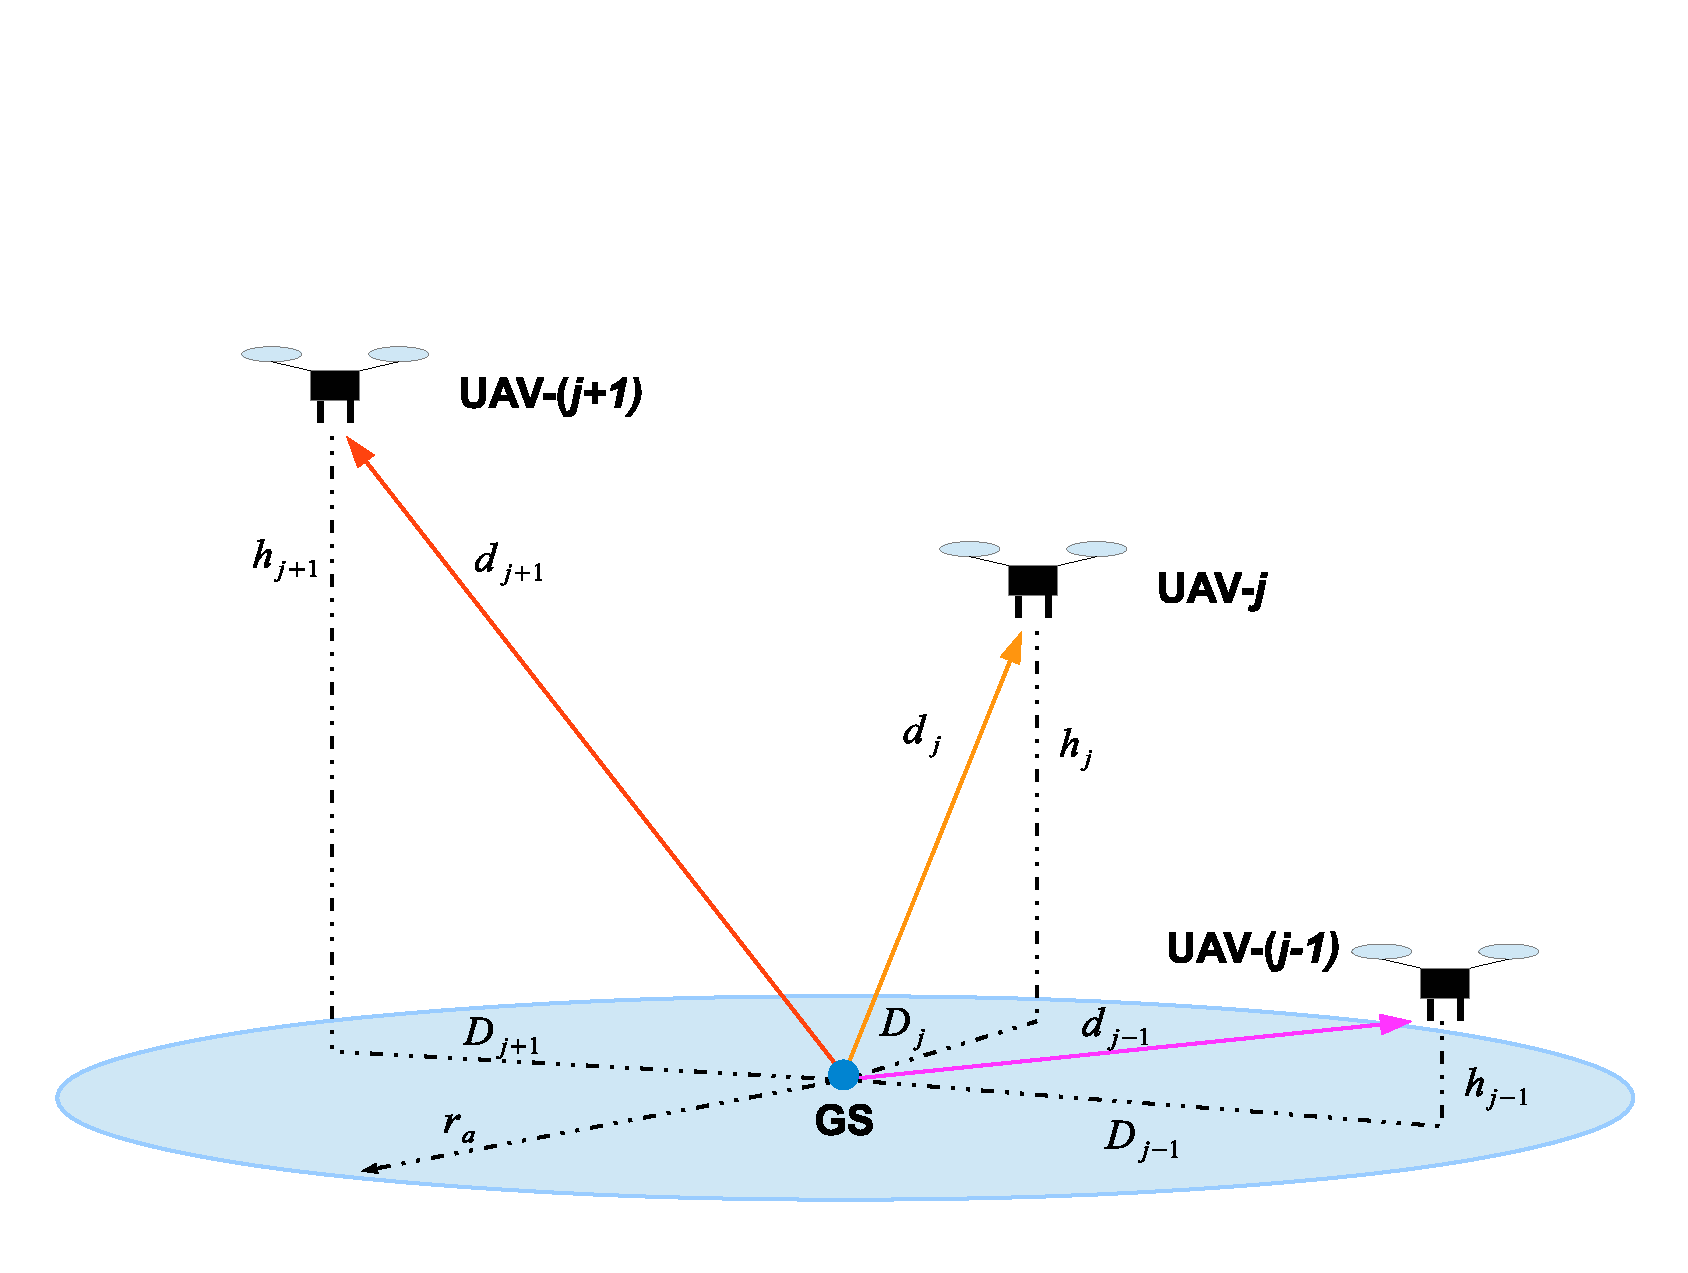
\includegraphics [width=0.6\columnwidth]{chap8_fig/block_diagram3.eps}
\caption{An illustration of the NOMA-aided UCS operating in a suburban environment. The GS employs downlink NOMA to transmit data to the UAVs equipped with two reception antennas. At the UAVs, selection combining is employed to recover the transmitted data from the GS.}
\label{fig:NOMA_bivariate_Rician_Shadowed_system_model}
\end{figure}

Consider a NOMA-aided UCS operating in a suburban environment, comprising one single-antenna GS and $N_D$ downlink UAVs equipped with two receive antennas (Fig. \ref{fig:NOMA_bivariate_Rician_Shadowed_system_model}). The GS in the NOMA-aided UCS employs downlink NOMA to transmit data, while selection combining is employed as the reception strategy at the $N_D$ downlink UAVs. However, due to insufficient spacing between the receive antennas at the UAVs and the relative position of the UAVs to the GS, the downlink NOMA transmissions are assumed to occur over correlated fading channels. Separately, based on studies in \cite{chetlur2017downlink} and \cite{wang2018modeling}, a BPP model is employed in the present work to account for the spatial locations of the UAVs. It is also assumed that the UAVs are operating at a minimum altitude of $h_{min}$ \cite{chetlur2017downlink,wang2018modeling}, with compensated Doppler shifts \cite{tan2018joint}. Lastly, as a suburban setting is considered in this work, the bivariate Rician shadowed fading model is assumed for the UAV channels to account for the correlation between the receive antennas at the downlink UAVs. \textcolor{black}{\footnote{\textcolor{black}{It is worth noting that the analytical approach in this paper is also extensible to multi-antenna selection combining receivers.}}} A summary of important notations is also given in Table \ref{table:NOMA_bivariate_Rician_Shadowed_summary_impt_notations}.

\subsection{Distribution of UAV Spatial Locations}

Let the spatial location of the UAVs follow a uniform distribution in a disc centered at origin $O$ above the GS with radius $r_a$ and angle $\left[0,2\pi\right)$. Then, the Euclidean distance (km) between downlink UAV-$j$ and the GS is $d_{j}=\sqrt{D_{j}^2 + h_j^2}$, where $1 \leq j \leq N_D$ is the index of downlink UAV-$j$, $D_{j}$ is the projected Euclidean distance on the ground plane between the GS and downlink UAV-$j$, $h_j = h_{min} + \omega \frac{j}{N_D}$ is the altitude of downlink UAV-$j$, $\omega>0$ is the altitude separation factor between the DL UAVs. 

As the spatial location of downlink UAV-$j$ follows a uniform distribution, the PDF $f_{d_{j}}(w)$ of $d_{j}$ is given as \cite[eq. (3)]{chetlur2017downlink}, \cite{ernest2019hybrid}:
%%%%%%%%%%%%%%%%%%%%%%%%%%%%%%%%%%%%%%%%%%%%%%%%%%%%%%%%%%%%%%%%%%%%%%%%%%%%%%%%%
\begin{eqnarray}
f_{d_{j}}(w) & = & \frac{2w}{r_a^2}_,
\end{eqnarray}
%%%%%%%%%%%%%%%%%%%%%%%%%%%%%%%%%%%%%%%%%%%%%%%%%%%%%%%%%%%%%%%%%%%%%%%%%%%%%%%%%
where $L_{m,j} \leq w \leq L_{p,j}$, $L_{m,j} = h_j$, and $L_{p,j} = \sqrt{h_j^2+r_{a}^2}$. Through the PDF $f_{d_{j}}(w)$, a performance analysis of correlated downlink NOMA transmissions can now be conducted with the spatial distribution of the UAVs taken into consideration.

\subsection{Instantaneous SINR at Downlink UAV-$j$}
Following downlink NOMA transmission principles, the GS uses superposition coding to transmit the SOI to all downlink UAVs. Specifically, an SIC detector is employed at downlink UAV-$j$ to detect the SOI in the presence of MUI from the SOIs of the other downlink UAVs. Let $R_{j,l}$ be the instantaneous channel envelope of the $l$th receive antenna at downlink UAV-$j$ for $l \in \{1,2\}$, where $R_{j,l}$ follows a bivariate Rician shadowed distribution. Then, the instantaneous SINR of the $l$th receive antenna at downlink UAV-$j$ $\big(SINR_{j,l}\big)$ is:
%%%%%%%%%%%%%%%%%%%%%%%%%%%%%%%%%%%%%%%%%%%%%%%%%%%%%%%%%%%%%%%%%%%%%%%%%%%%%%%%%
\begin{eqnarray}
SINR_{j,l} & = & \frac{P_r a_{j} d_j^{-L} |R_{j,l}|^2}{1 + P_r d_j^{-L} |R_{j,l}|^2 \sum_{i=1}^{j-1} a_i}
\end{eqnarray}
%%%%%%%%%%%%%%%%%%%%%%%%%%%%%%%%%%%%%%%%%%%%%%%%%%%%%%%%%%%%%%%%%%%%%%%%%%%%%%%%%
where $P_r \propto \frac{P_t}{P_L \eta}$ is the normalized average received power \cite{ernest2019outage}, $P_t$ is the transmit power of the GS, $P_L = \big(\frac{4 \pi \cdot 10^9}{3 \cdot 10^8} f_c\big)^2$, $L$ is the pathloss exponent, $\eta = -174 + 10\log_{10}(B_W)$ is the strength of the AWGN in dBm \cite{hou2019exploiting}, $f_c$ is the carrier frequency (MHz), $B_W$ is the bandwidth (Hz), and $a_j$ is the power allocation factor for DL UAV-$j$ such that $\sum_{j=1}^{N_D} \alpha_j = 1$.

It is useful to recall that the downlink UAVs operate at different altitudes, i.e., $H_{j} < H_{j+1}$. As such, the power allocation factor $a_j$ is heuristically defined based on the altitudes of the $N_D$ downlink UAVs to ensure fairness. Specifically, we let $a_j = \frac{H_j}{\sum_{k=1}^{N_D} H_k}$ in order to assign higher transmit powers to UAVs operating far away from the GS \cite{liu2018heterogeneous}, i.e., $a_j < a_{j+1}$. Doing so allows downlink UAV-$j$ to recover the SOI by performing SIC to remove MUI from downlink UAV-$m$ for $m>j$, while ignoring MUI from DL UAV-$k$ for $k<j$ \cite{salehi2019meta,islam2017power}.

\begin{table}[]
\centering
\caption{Summary of Important Notations}
\label{table:NOMA_bivariate_Rician_Shadowed_summary_impt_notations} 
\scalebox{0.8}{
\begin{tabular}{ll}
\hline
\textbf{Notations}		& \textbf{Description}																	\\  \hline \hline
$1 \leq j \leq N_D$		& Index of DL UAV-$j$																		\\ \hline
$h_{min}$; $\omega$		&	Minimum UAV altitude; Altitude separation factor			\\
$h_{j}$								&	Altitude of DL UAV-$j$																\\
$d_{j}$								& Euclidean distance between the GS and DL UAV-$j$			\\
$P_r$									& Normalized average received power											\\
$a_j$									& Power allocation factor for DL UAV-$j$ 								\\
$\rho$								& Cross correlation factor															\\
$m$ 									& Shaping parameter, denotes shadowing severity					\\
$\sigma^2$						& Varinace of bivariate Rician shadowed random variable	\\ \hline
\end{tabular}}
\end{table}
%A summary of important notations is also given in Table \ref{table:NOMA_bivariate_Rician_Shadowed_summary_impt_notations}.

%%%%%%%%%%%%%%%%%%%%%%%%%%%%%%%%%%%%%%%%%%%%%%%%%%%%%%%%%%%%%%%%%%%%%%%%%%%%%%%%%%%%%%%%%%%%%%%%%%%%%%%%%%%%%%%%%%%%%%%%%%%%%%%%%%%%%%%%%
% Section 3 : Bivariate Rician Shadowed Fading PDF Derivations
\section{Bivariate Rician Shadowed Fading Model} \label{NOMA_bivariate_Rician_Shadowed_sec_bi_var}

In UAV communications, correlation of the UAV channels can occur due to insufficient spacing between the UAV's receive antenna, the heading of the UAV, and the position of the UAV relative to the GS \cite{tan2019downlink,jiang2010dynamic,jin2017three,jiang2012optimization}. As such, we introduce the bivariate Rician shadowed fading model in this section as the basis to model the correlated UAV channels.

To begin, a pair of bivariate Rician shadowed distributed random variables RVs, $H_{1}$ and $H_{2}$, is modeled as \cite{lopez2018bivariate}:
%%%%%%%%%%%%%%%%%%%%%%%%%%%%%%%%%%%%%%%%%%%%%%%%%%%%%%%%%%%%%%%%%%%%%%%%%%%%%%%%%
\begin{eqnarray} \label{NOMA_bivariate_Rician_Shadowed_rv_bi_rician_shad}
H_k = \sigma\sqrt{1-\rho}X_k + \sigma\sqrt{\rho}X_0 + Z,
\end{eqnarray}
%%%%%%%%%%%%%%%%%%%%%%%%%%%%%%%%%%%%%%%%%%%%%%%%%%%%%%%%%%%%%%%%%%%%%%%%%%%%%%%%%
where $X_k, k \in \{0,1,2\}$ are Gaussian RVs with zero mean and variance $\frac{1}{2}$, $0 \leq \rho \leq 1$ is the cross correlation coefficient, $E\big\{ \big(\sigma\sqrt{1-\rho}X_k + \sigma\sqrt{\rho}X_0\big)^2 \big\} = \sigma^2$ \cite{lopez2018bivariate}, and $E\{\bullet\}$ is the statistical expectation operator. Finally, the RV $Z$ follows a Nakagami-$m$ distribution with shaping parameter $m\geq 0.5$ and $E\{|Z|^2\}=\Omega_N$.

\subsection{Derivation of the Joint PDF and Joint CDF}
Defining $R_k = |H_k|$, we note that the RV $R_k$ follows a bivariate Rician shadowed distribution with $E\{R_k^2\}=\sigma^2(1+K)$ and Rician factor $K=\frac{\Omega_N}{\sigma^2}$. From \cite[eq. (4)]{lopez2018bivariate}, the joint PDF $f_{R_1,R_2}(r_1,r_2)$ of $R_k$ is: 
%%%%%%%%%%%%%%%%%%%%%%%%%%%%%%%%%%%%%%%%%%%%%%%%%%%%%%%%%%%%%%%%%%%%%%%%%%%%%%%%%
\begin{eqnarray} \label{NOMA_bivariate_Rician_Shadowed_pdf_bi_rician_shad}
 f_{R_1,R_2}(r_1,r_2) & = & \frac{8 (\frac{m \rho}{m \rho + K})^m}{\sigma^6 \rho (1-\rho)^2} r_1 r_2 \exp\bigg(-\frac{r_1^2 + r_2^2}{\sigma^2(1-\rho)}\bigg) \nonumber \\
 & & \hspace{-2.5cm} \times \int_0^\infty x \exp\bigg( \frac{-(1+\rho)}{\sigma^2 \rho(1-\rho)}x^2 \bigg) I_0\bigg( \frac{2r_1x}{\sigma^2(1-\rho)} \bigg) I_0\bigg( \frac{2r_2x}{\sigma^2(1-\rho)} \bigg) \nonumber \\
 & & \hspace{0.8cm} \times {}_1{F_1}\bigg(m,1;\frac{K}{\sigma^2 \rho(\rho m + K)}x^2\bigg) dx_,
\end{eqnarray}
%%%%%%%%%%%%%%%%%%%%%%%%%%%%%%%%%%%%%%%%%%%%%%%%%%%%%%%%%%%%%%%%%%%%%%%%%%%%%%%%%
where $I_{0}\left(\bullet\right)$ is the modified Bessel function of the first kind with zero order \cite[eq. (9.6.10)]{abramowitz1964handbook} and ${}_1{F_1}(\bullet)$ is the confluent Hypergeometric function \cite{gradshteyn2014table}.

The joint PDF expression in (\ref{NOMA_bivariate_Rician_Shadowed_pdf_bi_rician_shad}) may require the use of complicated numerical methods when evaluating commonly used performance metrics, e.g., outage probability. We present an alternative closed-form expression for $f_{R_1,R_2}(r_1,r_2)$ in the following Lemma:
%%%%%%%%%%%%%%%%%%%%%%%%%%%%%%%%%%%%%%%%%%%%%%%%%%%%%%%%%%%%%%%%%%%%%%%%%%%%%%%%%
\begin{lemma} \label{NOMA_bivariate_Rician_Shadowed_lemma_pwr_srs_pdf_bi_rician_shad}
The closed-form expression for $f_{R_1,R_2}(r_1,r_2)$ can be expressed as the following power series:
\begin{eqnarray} \label{NOMA_bivariate_Rician_Shadowed_pwr_srs_pdf_bi_rician_shad}
f_{R_1,R_2}(r_1,r_2) \approx \sum_{k=0}^{K_{tr,1}} \sum_{i=0}^{k} \sum_{n=0}^{i} \alpha(k,i,n) r_1^{2n+1} r_2^{2(i-n)+1} \exp\bigg( -\frac{r_1^2 + r_2^2}{\sigma^2 (1-\rho)} \bigg)_,
\end{eqnarray}
%%%%%%%%%%%%%%%%%%%%%%%%%%%%%%%%%%%%%%%%%%%%%%%%%%%%%%%%%%%%%%%%%%%%%%%%%%%%%%%%%
\end{lemma}
where 
%%%%%%%%%%%%%%%%%%%%%%%%%%%%%%%%%%%%%%%%%%%%%%%%%%%%%%%%%%%%%%%%%%%%%%%%%%%%%%%%%
\begin{eqnarray}
\alpha(k,i,n) = \frac{8(m)_{k-i}\big( \frac{K}{\sigma^2 \rho (\rho m + K)} \big)^{k-i} \big(\frac{m\rho}{m\rho+K}\big)^m k!}{\Gamma^2(n+1)\Gamma^2(i-n+1)[\sigma^2 (1-\rho)]^{2i} (1)_{k-i} (k-i)! \sigma^6 \rho (1-\rho)^2 \cdot 2\big(\frac{1+\rho}{\sigma^2 \rho (1-\rho)}\big)^{k+1}}_, \nonumber
\end{eqnarray}
%%%%%%%%%%%%%%%%%%%%%%%%%%%%%%%%%%%%%%%%%%%%%%%%%%%%%%%%%%%%%%%%%%%%%%%%%%%%%%%%%
$K_{tr,j},j \in \{1,2\}$ is the truncation order, and $(a)_k=\frac{\Gamma(a+k)}{\Gamma(a)}$ is the Pochhammer symbol \cite[eq. (6.1.22)]{abramowitz1964handbook}.

\begin{proof}
The proof is provided in Appendix \ref{NOMA_bivariate_Rician_Shadowed_pdf_lemma_proof}
\end{proof}

As the subsequent analysis in the rest of this chapter are based on the power series expression in (\ref{NOMA_bivariate_Rician_Shadowed_pwr_srs_pdf_bi_rician_shad}), it is crucial to show that (\ref{NOMA_bivariate_Rician_Shadowed_pwr_srs_pdf_bi_rician_shad}) is convergent. In the next Corollary, we show that the alternative closed-form expression for $f_{R_1,R_2}(r_1,r_2)$ in (\ref{NOMA_bivariate_Rician_Shadowed_pwr_srs_pdf_bi_rician_shad}) is convergent.
%%%%%%%%%%%%%%%%%%%%%%%%%%%%%%%%%%%%%%%%%%%%%%%%%%%%%%%%%%%%%%%%%%%%%%%%%%%%%%%%%
\begin{corollary} \label{NOMA_bivariate_Rician_Shadowed_pdf_corollary_convergence}
The closed-form expression for $f_{R_1,R_2}(r_1,r_2)$ in (\ref{NOMA_bivariate_Rician_Shadowed_pwr_srs_pdf_bi_rician_shad}) has a convergence radius of $\infty$. 
\end{corollary}
\begin{proof}
The proof is given in Appendix \ref{NOMA_bivariate_Rician_Shadowed_pdf_corollary_convergence_proof}.
\end{proof}
%%%%%%%%%%%%%%%%%%%%%%%%%%%%%%%%%%%%%%%%%%%%%%%%%%%%%%%%%%%%%%%%%%%%%%%%%%%%%%%%%

As a result of Corollary \ref{NOMA_bivariate_Rician_Shadowed_pdf_corollary_convergence}, term-wise integration and differentiation can be performed on the power series expression in (\ref{NOMA_bivariate_Rician_Shadowed_pwr_srs_pdf_bi_rician_shad}) \cite{amann2005analysis,gradshteyn2014table}. Therefore, the closed-form joint CDF $F_{R_1,R_2}(\gamma_1,\gamma_2)$ can also be obtained from (\ref{NOMA_bivariate_Rician_Shadowed_pwr_srs_pdf_bi_rician_shad}) as shown in the following Lemma:
%%%%%%%%%%%%%%%%%%%%%%%%%%%%%%%%%%%%%%%%%%%%%%%%%%%%%%%%%%%%%%%%%%%%%%%%%%%%%%%%%
\begin{lemma} \label{NOMA_bivariate_Rician_Shadowed_lemma_pwr_srs_cdf_bi_rician_shad}
The closed-form expressions for $F_{R_1,R_2}(\gamma_1,\gamma_2)$ can be expressed as:
\begin{eqnarray} 
F_{R_1,R_2}(\gamma_1,\gamma_2)\approx \sum_{k=0}^{K_{tr,1}} \sum_{i=0}^{k} \sum_{n=0}^{i} \sum_{l=0}^{K_{tr,2}} \sum_{q=0}^{l} \alpha(k,i,n) G(l,n,i,q) (\gamma_1)^{2(q+n+1)} {(\gamma_2)^{2(l-q+i-n+1)}}_, \label{NOMA_bivariate_Rician_Shadowed_pwr_srs_cdf}
\end{eqnarray}
%%%%%%%%%%%%%%%%%%%%%%%%%%%%%%%%%%%%%%%%%%%%%%%%%%%%%%%%%%%%%%%%%%%%%%%%%%%%%%%%%
\end{lemma}
where $G(l,n,i,q) = \frac{(-1)^l \binom{l}{q}}{[\sigma^2(1-\rho)]^{l} l! 4 (q+n+1) (l-q+i-n+1)}$.

\begin{proof}
The proof is provided in Appendix \ref{NOMA_bivariate_Rician_Shadowed_cdf_lemma_proof}.
\end{proof}

Compared to the expression of $F_{R_1,R_2}(\gamma_1,\gamma_2)$ given in \cite[eq. (23)]{lopez2018bivariate}, (\ref{NOMA_bivariate_Rician_Shadowed_pwr_srs_cdf}) demonstrates that $F_{R_1,R_2}(\gamma_1,\gamma_2)$ can be evaluated in closed-form. Furthermore, (\ref{NOMA_bivariate_Rician_Shadowed_pwr_srs_cdf}) is presented in a desirable form, as term-wise integration and differentiation can be conducted using the presented power series expression. As it will be shown, (\ref{NOMA_bivariate_Rician_Shadowed_pwr_srs_cdf}) enables the tractable derivation of the NOMA-aided UCS outage probability and diversity gain under the BPP model, which may not be possible using \cite[eq. (23)]{lopez2018bivariate}.

\subsection{Truncation Analysis of the Joint PDF and Joint CDF}
It is worth noting that Corollary \ref{NOMA_bivariate_Rician_Shadowed_pdf_corollary_convergence} is evaluated by applying the D'Alembert test on $k$, $i$, and $n$ in (\ref{NOMA_bivariate_Rician_Shadowed_pwr_srs_pdf_bi_rician_shad}). Since the D'Alembert test indicates a convergence radius of $\infty$, the same technique can also be extended to determine the truncation error $\big(\mathcal{T}_{\epsilon}\big)$ of the joint PDF $f_{R_1,R_2}(r_1,r_2)$ in (\ref{NOMA_bivariate_Rician_Shadowed_pwr_srs_pdf_bi_rician_shad}). In particular, $\mathcal{T}_{\epsilon}$ can be defined as \cite[eq. (92)]{o2011product}:
%%%%%%%%%%%%%%%%%%%%%%%%%%%%%%%%%%%%%%%%%%%%%%%%%%%%%%%%%%%%%%%%%%%%%%%%%%%%%%%%%
\begin{eqnarray} \label{NOMA_bivariate_Rician_Shadowed_te}
\mathcal{T}_{\epsilon} & = & \sum_{k=K_{tr,1} + 1}^{\infty} \sum_{i=0}^{K_{tr,1}} \sum_{n=0}^{i} \alpha(k,i,n) \nonumber \\
 & & \hspace{1cm} \times r_1^{2n+1} r_2^{2(i-n)+1} \exp\bigg( -\frac{r_1^2 + r_2^2}{\sigma^2 (1-\rho)} \bigg)_.
\end{eqnarray}
%%%%%%%%%%%%%%%%%%%%%%%%%%%%%%%%%%%%%%%%%%%%%%%%%%%%%%%%%%%%%%%%%%%%%%%%%%%%%%%%%

From (\ref{NOMA_bivariate_Rician_Shadowed_te}), we present an upper bound of the truncation error $\big(\mathcal{T}_{\epsilon,upper}\big)$ for the joint PDF $f_{R_1,R_2}(r_1,r_2)$ in (\ref{NOMA_bivariate_Rician_Shadowed_pwr_srs_pdf_bi_rician_shad}) in the next Lemma:
%%%%%%%%%%%%%%%%%%%%%%%%%%%%%%%%%%%%%%%%%%%%%%%%%%%%%%%%%%%%%%%%%%%%%%%%%%%%%%%%%
\begin{lemma} \label{NOMA_bivariate_Rician_Shadowed_lemma_te_upper}
For a sufficiently large truncation order $\big(K_{tr,1}\big)$, the upper bound of the truncation error in (\ref{NOMA_bivariate_Rician_Shadowed_pwr_srs_pdf_bi_rician_shad}) is:
\begin{eqnarray} \label{NOMA_bivariate_Rician_Shadowed_te_upper}
\mathcal{T}_{\epsilon,upper} & = & \sum_{i=0}^{K_{tr,1}} \sum_{n=0}^{i} \frac{\alpha\big(K_{tr,1},i,n\big)}{1-\Delta\big(K_{tr,1}\big)} \nonumber \\
 & & \hspace{0.5cm} \times r_1^{2n+1} r_2^{2(i-n)+1} \exp\bigg( -\frac{r_1^2 + r_2^2}{\sigma^2 (1-\rho)} \bigg)_,
\end{eqnarray}
%%%%%%%%%%%%%%%%%%%%%%%%%%%%%%%%%%%%%%%%%%%%%%%%%%%%%%%%%%%%%%%%%%%%%%%%%%%%%%%%%
\end{lemma}
where $\Delta(k) = \Big( \frac{K}{\sigma^2 \rho (\rho m + K)} \Big)\frac{1}{k}$.

\begin{proof}
The proof is provided in Appendix \ref{NOMA_bivariate_Rician_Shadowed_lemma_te_upper_proof}
\end{proof}

The expression in (\ref{NOMA_bivariate_Rician_Shadowed_te_upper}) is useful in determining the necessary value of $K_{tr,1}$ that satisfies $\mathcal{T}_{\epsilon,upper} < \epsilon$, where $\epsilon$ is an error threshold value, for varying values of the Rician $K$ factor, $m$, $\sigma$, and $\rho$. From (\ref{NOMA_bivariate_Rician_Shadowed_te_upper}), the behavior of $\mathcal{T}_{\epsilon,upper}$ with respect to the Rician $K$ factor, $m$, $\sigma$, and $\rho$ is given in the following Corollaries:
%%%%%%%%%%%%%%%%%%%%%%%%%%%%%%%%%%%%%%%%%%%%%%%%%%%%%%%%%%%%%%%%%%%%%%%%%%%%%%%%%
\begin{corollary} \label{NOMA_bivariate_Rician_Shadowed_corollary_te_upper_behavior_m_rho_sigma}
Increasing $m$, $\sigma$, or $\rho$ leads to a smaller $\mathcal{T}_{\epsilon,upper}$.
\end{corollary}
\begin{proof}
From (\ref{NOMA_bivariate_Rician_Shadowed_te_upper}), it is noted that $m$, $\sigma$, and $\rho$ are in the denominator of $\Delta(k)$. Therefore, $\Delta(k) \to 0$ when $m$, $\sigma$, or $\rho$ is increased. This completes the proof.
\end{proof}
%%%%%%%%%%%%%%%%%%%%%%%%%%%%%%%%%%%%%%%%%%%%%%%%%%%%%%%%%%%%%%%%%%%%%%%%%%%%%%%%%
\begin{corollary} \label{NOMA_bivariate_Rician_Shadowed_corollary_te_upper_behavior_Rician_K_factor}
As the Rician $K$ factor increases, a sufficiently large $K_{tr,1}$ is needed in order to reduce $\mathcal{T}_{\epsilon,upper}$.
\end{corollary}
\begin{proof}
From (\ref{NOMA_bivariate_Rician_Shadowed_te_upper}), it is seen that $\lim_{k \to \infty} \Delta(k) = \frac{1}{k} \lim_{k \to \infty} \frac{K}{\sigma^2 \rho (\rho m + K)} = \frac{1}{k}$. Therefore, as the Rician $K$ factor increases, $\Delta(k) \to 0$ only when $K_{tr,1}$ is sufficiently large. This completes the proof.
\end{proof}
%%%%%%%%%%%%%%%%%%%%%%%%%%%%%%%%%%%%%%%%%%%%%%%%%%%%%%%%%%%%%%%%%%%%%%%%%%%%%%%%%

The impact of the Rician $K$ factor, $m$, $\sigma$, and $\rho$ on $\mathcal{T}_{\epsilon,upper}$ is established in Corollaries \ref{NOMA_bivariate_Rician_Shadowed_corollary_te_upper_behavior_m_rho_sigma} and \ref{NOMA_bivariate_Rician_Shadowed_corollary_te_upper_behavior_Rician_K_factor}. For instance, smaller $K_{tr,1}$ can be used when (\ref{NOMA_bivariate_Rician_Shadowed_pwr_srs_pdf_bi_rician_shad}) is used to model a bivariate Rayleigh shadowed fading environment, i.e., Rician $K$ factor is zero. Furthermore, Corollaries \ref{NOMA_bivariate_Rician_Shadowed_corollary_te_upper_behavior_m_rho_sigma} and \ref{NOMA_bivariate_Rician_Shadowed_corollary_te_upper_behavior_Rician_K_factor} can also be used to provide an indication of the necessary $K_{tr,1}$ for varying values of the Rician $K$ factor, $m$, $\sigma$, and $\rho$. 

The approach in Lemma \ref{NOMA_bivariate_Rician_Shadowed_lemma_te_upper} and Corollaries \ref{NOMA_bivariate_Rician_Shadowed_corollary_te_upper_behavior_m_rho_sigma} and \ref{NOMA_bivariate_Rician_Shadowed_corollary_te_upper_behavior_Rician_K_factor} can also be used to analyze the truncation error $\big(e\big)$ of the joint CDF $F_{R_1,R_2}(\gamma_1,\gamma_2)$ in (\ref{NOMA_bivariate_Rician_Shadowed_pwr_srs_cdf}). Specifically, $e$ can be defined as \cite[eq. (82)]{o2011product}:
%%%%%%%%%%%%%%%%%%%%%%%%%%%%%%%%%%%%%%%%%%%%%%%%%%%%%%%%%%%%%%%%%%%%%%%%%%%%%%%%%
\begin{eqnarray} \label{NOMA_bivariate_Rician_Shadowed_e}
e & = & \sum_{k=0}^{K_{tr}} \sum_{i=0}^{k} \sum_{n=0}^{i} \sum_{l=K_{tr}+1}^{\infty} \sum_{q=0}^{l} \mu(k,l) + \sum_{k=K_{tr}+1}^{\infty} \sum_{i=0}^{k} \sum_{n=0}^{i} \sum_{l=0}^{K_{tr}} \sum_{q=0}^{l} \mu(k,l) \nonumber \\
	& & + \sum_{k=K_{tr}+1}^{\infty} \sum_{i=0}^{k} \sum_{n=0}^{i} \sum_{l=k}^{\infty} \sum_{q=0}^{l} \mu(k,l) + \sum_{l=K_{tr}+1}^{\infty} \sum_{q=0}^{l} \sum_{k=l}^{\infty} \sum_{i=0}^{k} \sum_{n=0}^{i} \mu(k,l)_, 
\end{eqnarray}
%%%%%%%%%%%%%%%%%%%%%%%%%%%%%%%%%%%%%%%%%%%%%%%%%%%%%%%%%%%%%%%%%%%%%%%%%%%%%%%%%
where $K_{tr,1} = K_{tr,2} = K_{tr}$ and $\mu(k,l) = \alpha(k,i,n) G(l,n,i,q) (\gamma_1)^{2(q+n+1)} (\gamma_2)^{2(l-q+i-n+1)}$. From (\ref{NOMA_bivariate_Rician_Shadowed_e}), the upper bound of the truncation error $\big(e_{upper}\big)$ for the joint CDF $F_{R_1,R_2}(\gamma_1,\gamma_2)$ in (\ref{NOMA_bivariate_Rician_Shadowed_pwr_srs_cdf}) is presented in the next Lemma:
%%%%%%%%%%%%%%%%%%%%%%%%%%%%%%%%%%%%%%%%%%%%%%%%%%%%%%%%%%%%%%%%%%%%%%%%%%%%%%%%%
\begin{lemma} \label{NOMA_bivariate_Rician_Shadowed_lemma_e_upper}
For a sufficiently large truncation order $\big(K_{tr}\big)$, the upper bound of the truncation error in (\ref{NOMA_bivariate_Rician_Shadowed_pwr_srs_cdf}) is:
\begin{eqnarray} \label{NOMA_bivariate_Rician_Shadowed_e_upper}
e_{upper} & = & \sum_{k=0}^{K_{tr}} \sum_{i=0}^{k} \sum_{n=0}^{i} \sum_{q=0}^{K_{tr}+1} \frac{\mu(k,K_{tr}+1)}{1-\Theta_1(k,K_{tr}+1)} + \sum_{i=0}^{K_{tr}} \sum_{n=0}^{i} \sum_{l=0}^{K_{tr}} \sum_{q=0}^{l} \frac{\mu(K_{tr},l)}{1-\Theta_2(K_{tr})} \nonumber \\
	& & \hspace{-1cm} + \sum_{k=K_{tr}+1}^{\infty} \sum_{i=0}^{k} \sum_{n=0}^{i} \sum_{q=0}^{K_{tr}+1} \frac{\mu(k,K_{tr}+1)}{1-\Theta_1(k,K_{tr}+1)} + \sum_{q=0}^{K_{tr}+1} \sum_{i=0}^{K_{tr}} \sum_{n=0}^{i} {\frac{\mu(K_{tr},K_{tr}+1)}{1-\Theta_2(K_{tr})}}_, 
\end{eqnarray}
%%%%%%%%%%%%%%%%%%%%%%%%%%%%%%%%%%%%%%%%%%%%%%%%%%%%%%%%%%%%%%%%%%%%%%%%%%%%%%%%%
\end{lemma}
where $\Theta_1(k,l) = \frac{(-1) (\gamma_2)^2 (l+1) (l-q+i-n+1)}{\sigma^2(1-\rho) l^2 (l-q+i-n+2)}$ and $\Theta_2 (k) = \Delta(k) = \Big( \frac{K}{\sigma^2 \rho (\rho m + K)} \Big)\frac{1}{k}$.

\begin{proof}
The proof is provided in Appendix \ref{NOMA_bivariate_Rician_Shadowed_lemma_e_upper_proof}
\end{proof}

Similar to (\ref{NOMA_bivariate_Rician_Shadowed_te_upper}), the upper bound in (\ref{NOMA_bivariate_Rician_Shadowed_lemma_e_upper}) can be used to identify the necessary value of $K_{tr}$ such that $e_{upper} < \epsilon$, where $\epsilon$ is an error threshold value, for varying values of the Rician $K$ factor, $m$, $\sigma$, $\rho$, and $\gamma_2$. From (\ref{NOMA_bivariate_Rician_Shadowed_e_upper}), the behavior of $e_{upper}$ with respect to $\rho$ and $\gamma_2$ is given in the following Corollary:
%%%%%%%%%%%%%%%%%%%%%%%%%%%%%%%%%%%%%%%%%%%%%%%%%%%%%%%%%%%%%%%%%%%%%%%%%%%%%%%%%
\begin{corollary} \label{NOMA_bivariate_Rician_Shadowed_corollary_e_upper_behavior_rho_gamma}
Increasing $\rho$ or decreasing $\gamma_2$ leads to a smaller $e_{upper}$.
\end{corollary}
\begin{proof}
From (\ref{NOMA_bivariate_Rician_Shadowed_e_upper}), it is noted that $\rho$ is in the denominator of $\Theta_1(k,l)$. Likewise,$\gamma_2$ is in the numerator of $\Theta_1(k,l)$. Therefore, $\Theta_1(k,l) \to 0$ when $\rho$ is increased or when $\gamma_2$ is decreased. This completes the proof.
\end{proof}
%%%%%%%%%%%%%%%%%%%%%%%%%%%%%%%%%%%%%%%%%%%%%%%%%%%%%%%%%%%%%%%%%%%%%%%%%%%%%%%%%

The impact of $\rho$ and $\gamma_2$ on $e_{upper}$ is established in Corollary \ref{NOMA_bivariate_Rician_Shadowed_corollary_e_upper_behavior_rho_gamma}. Hence, one can now use Corollary \ref{NOMA_bivariate_Rician_Shadowed_corollary_e_upper_behavior_rho_gamma} to decide on the choice of $K_{tr}$ to obtain $e_{upper} < \epsilon$ based on $\rho$ and $\gamma_2$. It should also be noted that Corollaries \ref{NOMA_bivariate_Rician_Shadowed_corollary_te_upper_behavior_m_rho_sigma} and \ref{NOMA_bivariate_Rician_Shadowed_corollary_te_upper_behavior_Rician_K_factor} are also applicable to (\ref{NOMA_bivariate_Rician_Shadowed_e_upper}). 


%%%%%%%%%%%%%%%%%%%%%%%%%%%%%%%%%%%%%%%%%%%%%%%%%%%%%%%%%%%%%%%%%%%%%%%%%%%%%%%%%%%%%%%%%%%%%%%%%%%%%%%%%%%%%%%%%%%%%%%%%%%%%%%%%%%%%%%%%
% Section 4 : Outage Probability Derivations
\section{Outage Probability Derivations} \label{NOMA_bivariate_Rician_Shadowed_sec_outage}

In this section, the downlink NOMA outage probability expression for downlink UAV-$j$ employing selection combining is presented. The OMA outage probability expression for downlink UAV-$j$ is also provided as a benchmark. Let the transmission rate of the GS be defined as $\mathcal{R}^{x}$, where $x \in \{NOMA, OMA\}$. For a fair comparison between NOMA and OMA, we let $\mathcal{R}^{NOMA}=\frac{1}{N_D}\mathcal{R}^{OMA}$.

%%%%%%%%%%%%%%%%%%%%%%%%%%%%%%%%%%%%%%%%%%%%%%%%%%%%%%%%%%%%%%%%%%%%%%%%%%%%%%%%%%%%%%%%%%%%%%%%%%%%%%%%%%%%%%%%%%%%%%%%%%%%%%%%%%%%%%%%%
\subsection{Downlink NOMA Outage Probability}

At downlink UAV-$j$, let the selection combining NOMA outage event $\big(\mathcal{O}_{j}^{NOMA}\big)$ be defined as:
%%%%%%%%%%%%%%%%%%%%%%%%%%%%%%%%%%%%%%%%%%%%%%%%%%%%%%%%%%%%%%%%%%%%%%%%%%%%%%%%%
\begin{eqnarray}
\mathcal{O}_{j}^{NOMA} = \Bigg\{ R_{j,l}, d_{j} : \max\big(R_{j,1},R_{j,2}\big) < \gamma_j^{NOMA} \sqrt{\frac{d_{j}^{L}}{P_r}}\Bigg\}_,
\end{eqnarray}
%%%%%%%%%%%%%%%%%%%%%%%%%%%%%%%%%%%%%%%%%%%%%%%%%%%%%%%%%%%%%%%%%%%%%%%%%%%%%%%%%
where $\gamma_j^{NOMA} = \sqrt{\frac{2^{\mathcal{R}^{NOMA}}-1}{a_{j} - \big(\sum_{i=1}^{j-1} a_i\big)\big(2^{\mathcal{R}^{NOMA}}-1\big)}}$ is the NOMA threshold such that $R^{NOMA} < \log_2\bigg(1 + \frac{a_{j}}{\sum_{i=1}^{j-1} a_i}\bigg)$. Then, the closed-form downlink NOMA outage probability expression for UAV-$j$ is presented in the following Theorem.

\begin{theorem} \label{NOMA_bivariate_Rician_Shadowed_theorem_P_out_down_uav}
%%%%%%%%%%%%%%%%%%%%%%%%%%%%%%%%%%%%%%%%%%%%%%%%%%%%%%%%%%%%%%%%%%%%%%%%%%%%%%%%%
The NOMA outage probability at downlink UAV-$j$ is:
\begin{eqnarray}
Pr\big(\mathcal{O}_{j}^{NOMA}\big) \approx \sum_{k=0}^{K_{tr,1}} \sum_{i=0}^{k} \sum_{n=0}^{i} \sum_{l=0}^{K_{tr,2}} \sum_{q=0}^{l} \alpha(k,i,n) G(l,n,i,q) \Xi_j\big(l,i\big) \Bigg[\frac{\big(\gamma_j^{NOMA}\big)^2}{P_r}\Bigg]^{2+l+i}_, \label{NOMA_bivariate_Rician_Shadowed_P_out_down_uav_j}
\end{eqnarray}
%%%%%%%%%%%%%%%%%%%%%%%%%%%%%%%%%%%%%%%%%%%%%%%%%%%%%%%%%%%%%%%%%%%%%%%%%%%%%%%%%
\end{theorem}
where $\Xi_j\big(l,i\big) = \frac{2 \big[ \big(L_{p,j}\big)^{L(2+l+i)+2} - \big(L_{m,j}\big)^{L(2+l+i)+2} \big]}{r_a^2[L(2+l+i)+2]}$.

\begin{proof}
The proof is provided in Appendix \ref{NOMA_bivariate_Rician_Shadowed_theorem_P_out_down_uav_proof}.
\end{proof}

%\begin{remark}
%\emph{It is worth emphasizing that the .}
%\end{remark}

In Theorem \ref{NOMA_bivariate_Rician_Shadowed_theorem_P_out_down_uav}, the effects of correlation, shadowing, and the Rician $K$ factors on the SOIs at the UAVs are mostly captured in the functions $\alpha(k,i,n)$ and $G(l,n,i,q)$. Similarly, the effects of the GS transmission rate and NOMA power allocation factor on outage probability are reflected in $\gamma_j^{NOMA}$, while the function $\Xi_j\big(l,i\big)$ in Theorem \ref{NOMA_bivariate_Rician_Shadowed_theorem_P_out_down_uav} captures the stochastic geometry behavior of the UAV spatial locations. Thus, using Theorem \ref{NOMA_bivariate_Rician_Shadowed_theorem_P_out_down_uav}, the reliability of downlink NOMA can be analyzed within the BPP model for UCSs. 

It is also worth emphasizing that the normalized average received power $(P_r)$ appears in the denominator of (\ref{NOMA_bivariate_Rician_Shadowed_P_out_down_uav_j}). As it will be shown subsequently, (\ref{NOMA_bivariate_Rician_Shadowed_P_out_down_uav_j}) indicates the absence of an outage probability error floor in $Pr\big(\mathcal{O}_{j}^{NOMA}\big)$ for downlink NOMA over correlated Rician shadowed fading channels.

%%%%%%%%%%%%%%%%%%%%%%%%%%%%%%%%%%%%%%%%%%%%%%%%%%%%%%%%%%%%%%%%%%%%%%%%%%%%%%%%%%%%%%%%%%%%%%%%%%%%%%%%%%%%%%%%%%%%%%%%%%%%%%%%%%%%%%%%%
\subsection{Downlink OMA Outage Probability}

As compared to NOMA, the GS transmits data to the downlink UAVs over separate time-frequency resources in OMA transmission schemes. Let the instantaneous SNR of the $l$th receive antenna at downlink UAV-$j$ be $SNR_{j,l} = P_r d_j^{-L} |R_{j,l}|^2$. Also, let the selection combining OMA outage event $\big(\mathcal{O}_{j}^{OMA}\big)$ be defined as:
%%%%%%%%%%%%%%%%%%%%%%%%%%%%%%%%%%%%%%%%%%%%%%%%%%%%%%%%%%%%%%%%%%%%%%%%%%%%%%%%%
\begin{eqnarray}
\mathcal{O}_{j}^{OMA} = \Bigg\{ R_{j,l}, d_{j} : \max\big(R_{j,1},R_{j,2}\big) < \gamma_j^{OMA} \sqrt{\frac{d_{j}^{L}}{P_r}}\Bigg\}_,
\end{eqnarray}
%%%%%%%%%%%%%%%%%%%%%%%%%%%%%%%%%%%%%%%%%%%%%%%%%%%%%%%%%%%%%%%%%%%%%%%%%%%%%%%%%
where $\gamma_j^{OMA} = \sqrt{2^{\mathcal{R}^{OMA}}-1}$ is the OMA threshold. Then, the closed-form OMA outage probability expression for UAV-$j$ is given in the next Theorem.

\begin{theorem} \label{NOMA_bivariate_Rician_Shadowed_theorem_P_out_oma_uav_j}
%%%%%%%%%%%%%%%%%%%%%%%%%%%%%%%%%%%%%%%%%%%%%%%%%%%%%%%%%%%%%%%%%%%%%%%%%%%%%%%%%
The OMA outage probability at downlink UAV-$j$ is:
%%%%%%%%%%%%%%%%%%%%%%%%%%%%%%%%%%%%%%%%%%%%%%%%%%%%%%%%%%%%%%%%%%%%%%%%%%%%%%%%%
\begin{eqnarray} 
Pr\big(\mathcal{O}_{j}^{OMA}\big) \approx \sum_{k=0}^{K_{tr,1}} \sum_{i=0}^{k} \sum_{n=0}^{i} \sum_{l=0}^{K_{tr,2}} \sum_{q=0}^{l} \alpha(k,i,n) G(l,n,i,q) \Xi_j\big(l,i\big) \Bigg[\frac{\big(\gamma_j^{OMA}\big)^2}{P_r}\Bigg]^{2+l+i}_. \label{NOMA_bivariate_Rician_Shadowed_P_out_oma_uav_j}
\end{eqnarray}
%%%%%%%%%%%%%%%%%%%%%%%%%%%%%%%%%%%%%%%%%%%%%%%%%%%%%%%%%%%%%%%%%%%%%%%%%%%%%%%%%
\end{theorem}
\begin{proof}
The expression in (\ref{NOMA_bivariate_Rician_Shadowed_P_out_oma_uav_j}) is obtained using the same approach in Appendix \ref{NOMA_bivariate_Rician_Shadowed_theorem_P_out_down_uav_proof}.
\end{proof}

Although one can also invoke \cite[eq. (48)]{lopez2018bivariate} to evaluate $Pr\big(\mathcal{O}_{j}^{OMA}\big)$, tractable analytical expressions may not be possible once the BPP model is considered. In contrast, we demonstrate in (\ref{NOMA_bivariate_Rician_Shadowed_P_out_oma_uav_j}) that evaluating $Pr\big(\mathcal{O}_{j}^{OMA}\big)$ within the BPP model can be achieved in a straightforward fashion using Lemma \ref{NOMA_bivariate_Rician_Shadowed_lemma_pwr_srs_cdf_bi_rician_shad}.

%%%%%%%%%%%%%%%%%%%%%%%%%%%%%%%%%%%%%%%%%%%%%%%%%%%%%%%%%%%%%%%%%%%%%%%%%%%%%%%%%%%%%%%%%%%%%%%%%%%%%%%%%%%%%%%%%%%%%%%%%%%%%%%%%%%%%%%%%
% Section 5 : Finite SNR Diversity Gain Derivations
\section{Finite SNR Diversity Gain Derivations} \label{NOMA_bivariate_Rician_Shadowed_sec_finite_SNR_diversity_gain}
The finite SNR diversity gain expressions for downlink NOMA and uplink NOMA are presented in this section. We also present finite SNR diversity gain expressions for OMA in this section.

The finite SNR diversity gain $d_f$ of a given system quantifies the decay of outage probability at low to moderate SNR regimes \cite{narasimhan2006finite,shin2008diversity}. In particular, the finite SNR diversity gain is defined as \cite[eq. (5)]{narasimhan2006finite}:
%%%%%%%%%%%%%%%%%%%%%%%%%%%%%%%%%%%%%%%%%%%%%%%%%%%%%%%%%%%%%%%%%%%%%%%%%%%%%%%%%
\begin{eqnarray} \label{NOMA_bivariate_Rician_Shadowed_df}
d_f & = & \frac{-P_r}{Pr\big(\mathcal{O}\big)}\frac{\partial}{\partial P_r}Pr\big(\mathcal{O}\big)_,
\end{eqnarray}
%%%%%%%%%%%%%%%%%%%%%%%%%%%%%%%%%%%%%%%%%%%%%%%%%%%%%%%%%%%%%%%%%%%%%%%%%%%%%%%%%
where $\mathcal{O}$ and $Pr\big(\mathcal{O}\big)$ are the considered outage event and outage probability, respectively. From \cite{shin2008diversity} and \cite{heidarpour2017finite}, one obtains the asymptotic diversity gain, defined in \cite{zheng2003diversity}, by evaluating (\ref{NOMA_bivariate_Rician_Shadowed_df}) at high SNR regimes. In this spirit, finite SNR analysis is employed to investigate the impact of MUI in downlink NOMA for UAV communications.

%%%%%%%%%%%%%%%%%%%%%%%%%%%%%%%%%%%%%%%%%%%%%%%%%%%%%%%%%%%%%%%%%%%%%%%%%%%%%%%%%%%%%%%%%%%%%%%%%%%%%%%%%%%%%%%%%%%%%%%%%%%%%%%%%%%%%%%%%
\subsection{Downlink NOMA Finite SNR Diversity Gain}

Let the downlink NOMA finite SNR diversity gain at UAV-$j$ be $d_{f,j}^{NOMA}$. Then, the closed-form expression for $d_{f,j}^{NOMA}$ is presented in the following Proposition.

\begin{proposition} \label{NOMA_bivariate_Rician_Shadowed_proposition_df_noma_uav_j}
%%%%%%%%%%%%%%%%%%%%%%%%%%%%%%%%%%%%%%%%%%%%%%%%%%%%%%%%%%%%%%%%%%%%%%%%%%%%%%%%%
The downlink NOMA finite SNR diversity gain at UAV-$j$ is:
\begin{eqnarray}
d_{f,j}^{NOMA} & \approx & \frac{-P_r}{Pr\big(\mathcal{O}_{j}^{NOMA}\big)} \sum_{k=0}^{K_{tr,1}} \sum_{i=0}^{k} \sum_{n=0}^{i} \sum_{l=0}^{K_{tr,2}} \sum_{q=0}^{l} \alpha(k,i,n) \nonumber \\
 & & \hspace{1cm} \times G(l,n,i,q) \Xi_j\big(l,i\big) \frac{\big(\gamma_j^{NOMA}\big)^{2(2+l+i)} (-2-l-i)}{(P_r)^{3+l+i}}_. \label{NOMA_bivariate_Rician_Shadowed_df_noma_uav_j}
\end{eqnarray}
%%%%%%%%%%%%%%%%%%%%%%%%%%%%%%%%%%%%%%%%%%%%%%%%%%%%%%%%%%%%%%%%%%%%%%%%%%%%%%%%%
\end{proposition}
\begin{proof}
Equation (\ref{NOMA_bivariate_Rician_Shadowed_df_noma_uav_j}) can be obtained from (\ref{NOMA_bivariate_Rician_Shadowed_P_out_down_uav_j}) by applying (\ref{NOMA_bivariate_Rician_Shadowed_df}). It should be noted that the differentiation conducted as a result of deriving (\ref{NOMA_bivariate_Rician_Shadowed_df_noma_uav_j}) is valid due to Corollary \ref{NOMA_bivariate_Rician_Shadowed_pdf_corollary_convergence} \cite{amann2005analysis,gradshteyn2014table}.
\end{proof}

As (\ref{NOMA_bivariate_Rician_Shadowed_P_out_down_uav_j}) is presented in a desirable form, i.e., as a power series, one can obtain a closed-form expression of $d_{f,j}^{NOMA}$ in (\ref{NOMA_bivariate_Rician_Shadowed_df_noma_uav_j}), which may not be tractable using the expression in \cite[eq. (48)]{lopez2018bivariate}. Furthermore, the expression in (\ref{NOMA_bivariate_Rician_Shadowed_df_noma_uav_j}) quantifies the NOMA outage probability decay of downlink UAV-$j$ as a function of $P_r$. Thus, a larger $d_{f,j}^{NOMA}$ indicates a steeper drop in $Pr\big(\mathcal{O}_{j}^{NOMA}\big)$ as $P_r$ varies. 

Using Proposition \ref{NOMA_bivariate_Rician_Shadowed_proposition_df_noma_uav_j}, one also arrives at the asymptotic NOMA diversity gain for downlink UAV-$j$ in the following Corollary.
%%%%%%%%%%%%%%%%%%%%%%%%%%%%%%%%%%%%%%%%%%%%%%%%%%%%%%%%%%%%%%%%%%%%%%%%%%%%%%%%%
\begin{corollary} \label{NOMA_bivariate_Rician_Shadowed_corollary_df_noma_uav_j}
At asymptotic SNR regimes, NOMA achieves full diversity gain at downlink UAV-$j$, i.e., $d_{f,j}^{NOMA}=2$.
%%%%%%%%%%%%%%%%%%%%%%%%%%%%%%%%%%%%%%%%%%%%%%%%%%%%%%%%%%%%%%%%%%%%%%%%%%%%%%%%%
\end{corollary}
\begin{proof}
The proof is provided in Appendix \ref{NOMA_bivariate_Rician_Shadowed_corollary_df_noma_uav_j_proof}. 
\end{proof}

Corollary \ref{NOMA_bivariate_Rician_Shadowed_corollary_df_noma_uav_j} shows that the NOMA-aided UCS is not interference-limited when employing downlink NOMA, despite the presence of MUI from the SOIs of other downlink UAVs. Furthermore, $d_{f,j}^{NOMA}$ is not affected by $\rho$ at high $P_t$ regimes.

%%%%%%%%%%%%%%%%%%%%%%%%%%%%%%%%%%%%%%%%%%%%%%%%%%%%%%%%%%%%%%%%%%%%%%%%%%%%%%%%%%%%%%%%%%%%%%%%%%%%%%%%%%%%%%%%%%%%%%%%%%%%%%%%%%%%%%%%%
\subsection{Downlink OMA Finite SNR Diversity Gain}

Let the downlink OMA finite SNR diversity gain at UAV-$j$ be $d_{f,j}^{OMA}$. Then, the closed-form expression for $d_{f,j}^{OMA}$ is presented in the following Proposition.

\begin{proposition} \label{NOMA_bivariate_Rician_Shadowed_proposition_df_oma_uav_j}
%%%%%%%%%%%%%%%%%%%%%%%%%%%%%%%%%%%%%%%%%%%%%%%%%%%%%%%%%%%%%%%%%%%%%%%%%%%%%%%%%
The downlink OMA finite SNR diversity gain at UAV-$j$ is:
\begin{eqnarray} 
d_{f,j}^{OMA} & \hspace{0cm} \approx & \hspace{0cm} \frac{-P_r}{Pr\big(\mathcal{O}_{j}^{OMA}\big)} \sum_{k=0}^{K_{tr,1}} \sum_{i=0}^{k} \sum_{n=0}^{i} \sum_{l=0}^{K_{tr,2}} \sum_{q=0}^{l} \alpha(k,i,n) \nonumber \\
 & & \hspace{1cm} \times G(l,n,i,q) \Xi_j\big(l,i\big) \frac{\big(\gamma_j^{OMA}\big)^{2(2+l+i)}(-2-l-i)}{(P_r)^{3+l+i}}_. \label{NOMA_bivariate_Rician_Shadowed_df_oma_uav_j}
\end{eqnarray}
%%%%%%%%%%%%%%%%%%%%%%%%%%%%%%%%%%%%%%%%%%%%%%%%%%%%%%%%%%%%%%%%%%%%%%%%%%%%%%%%%
\end{proposition}
\begin{proof}
The closed-form expression in (\ref{NOMA_bivariate_Rician_Shadowed_df_oma_uav_j}) is obtained using the same approach in Appendix \ref{NOMA_bivariate_Rician_Shadowed_corollary_df_noma_uav_j_proof}. 
\end{proof}

\begin{figure} [t] 
\centering
%\vspace{-1cm}
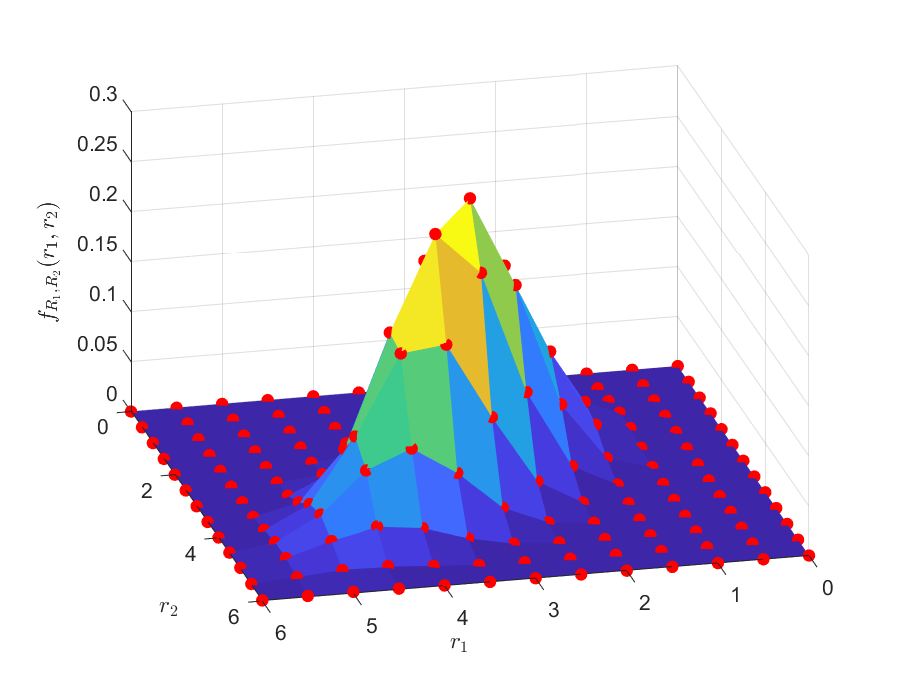
\includegraphics [width=0.6\columnwidth]{chap8_fig/pdf_comparison_edited.eps} 
%\vspace{-0.5cm}
\caption{Joint PDF comparison between the exact expression in (\ref{NOMA_bivariate_Rician_Shadowed_pdf_bi_rician_shad}) (denoted in red markers) and the closed-form expression in (\ref{NOMA_bivariate_Rician_Shadowed_pwr_srs_pdf_bi_rician_shad}) for $m=10$, $K_{tr,1}=150$, and Rician $K$ factor of 10 dB.}
%\vspace{-0.2cm}
\label{fig:NOMA_bivariate_Rician_Shadowed_pdf_comp}
\end{figure}

\begin{figure*}[t]
\centering
\subfloat[Impact of the Rician $K$ factor on $\mathcal{T}_{\epsilon,upper}$.]{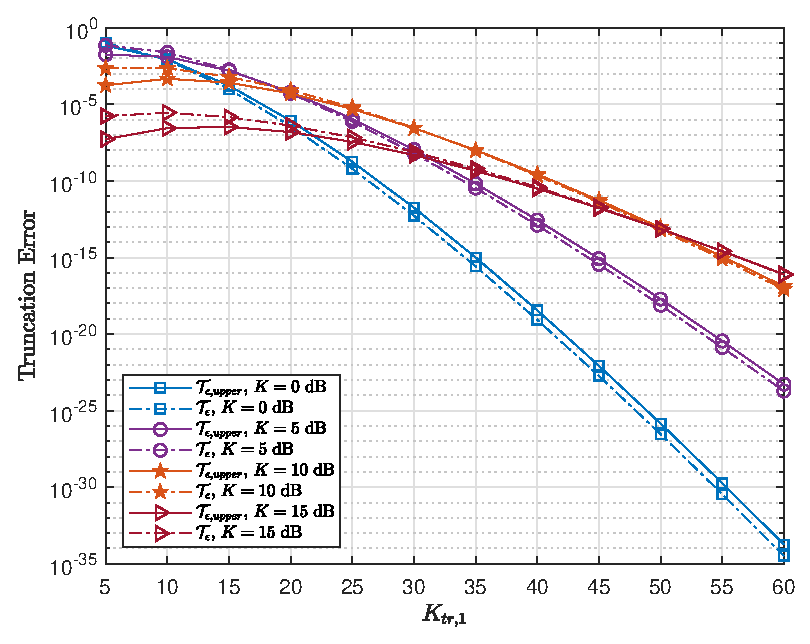
\includegraphics [width=0.45\columnwidth]{chap8_fig/k_factor_truncation_error.eps}
\label{fig:NOMA_bivariate_Rician_Shadowed_k_factor_truncation_error}} \vspace{0.1cm}
\hfil
\subfloat[Impact of $m$ on $\mathcal{T}_{\epsilon,upper}$.]{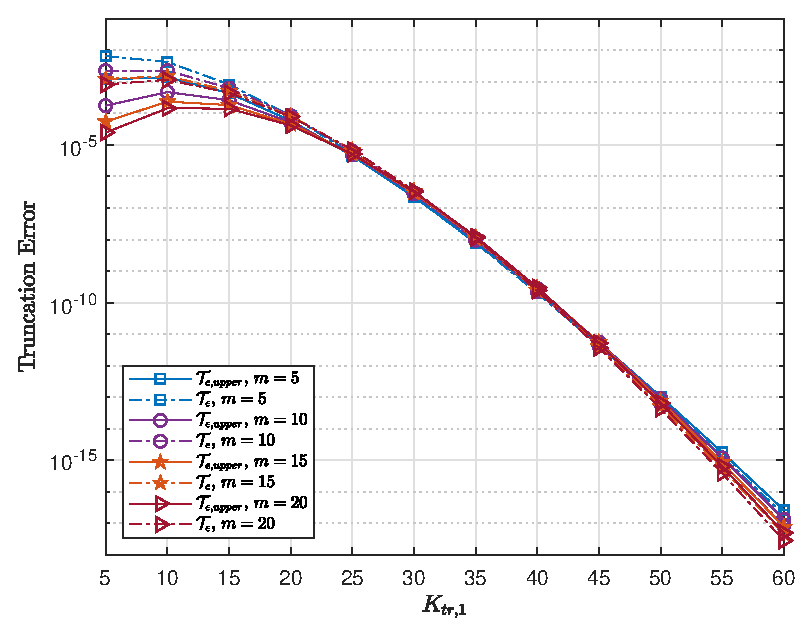
\includegraphics [width=0.45\columnwidth]{chap8_fig/shadowing_truncation_error.eps}
\label{fig:NOMA_bivariate_Rician_Shadowed_shadowing_truncation_error}} \vspace{0.1cm}
\hfil
\subfloat[Impact of $\sigma$ factor on $\mathcal{T}_{\epsilon,upper}$.]{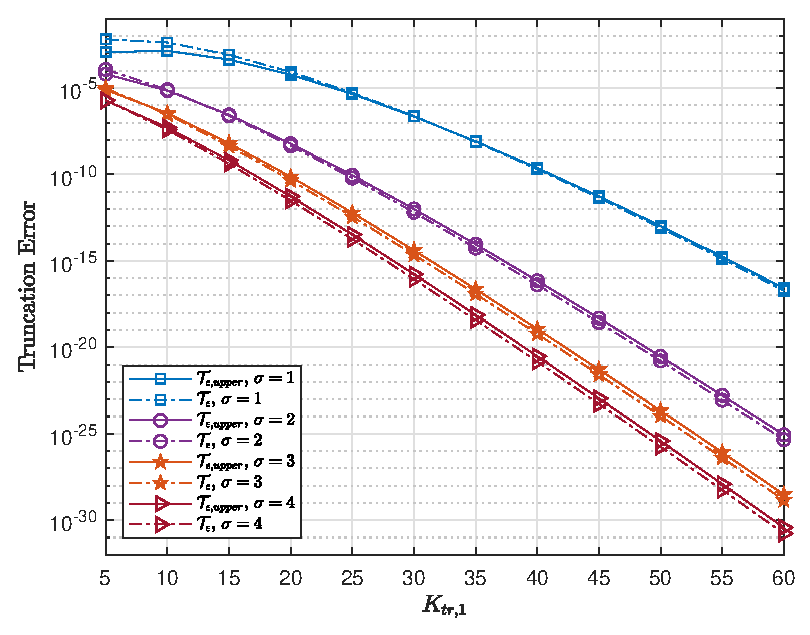
\includegraphics [width=0.45\columnwidth]{chap8_fig/sigma_truncation_error.eps}
\label{fig:NOMA_bivariate_Rician_Shadowed_sigma_truncation_error}} \vspace{0.1cm}
\hfil
\subfloat[Impact of $\rho$ on $\mathcal{T}_{\epsilon,upper}$.]{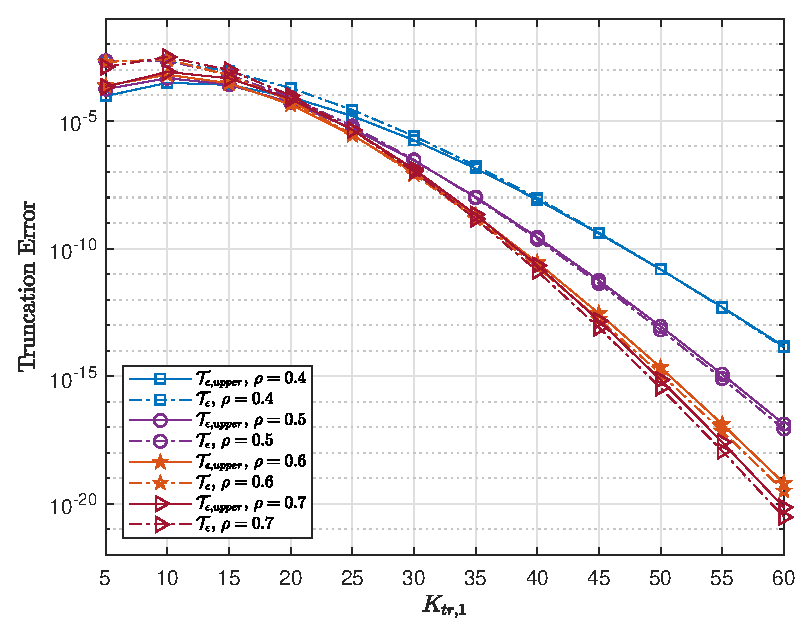
\includegraphics [width=0.45\columnwidth]{chap8_fig/rho_truncation_error.eps}
\label{fig:NOMA_bivariate_Rician_Shadowed_rho_truncation_error}} \vspace{0.1cm}
\caption{Impact of the Rician $K$ factor, $m$, $\sigma$, and $\rho$ on $\mathcal{T}_{\epsilon,upper}$ for $r_1 = r_2 = 1$ and Rician $K$ factor of 10 dB.}
\label{fig:NOMA_bivariate_Rician_Shadowed_truncation_error}
%\vspace{-0.51cm}
\end{figure*}

\begin{figure} [t] 
\centering
\vspace{0.5cm}
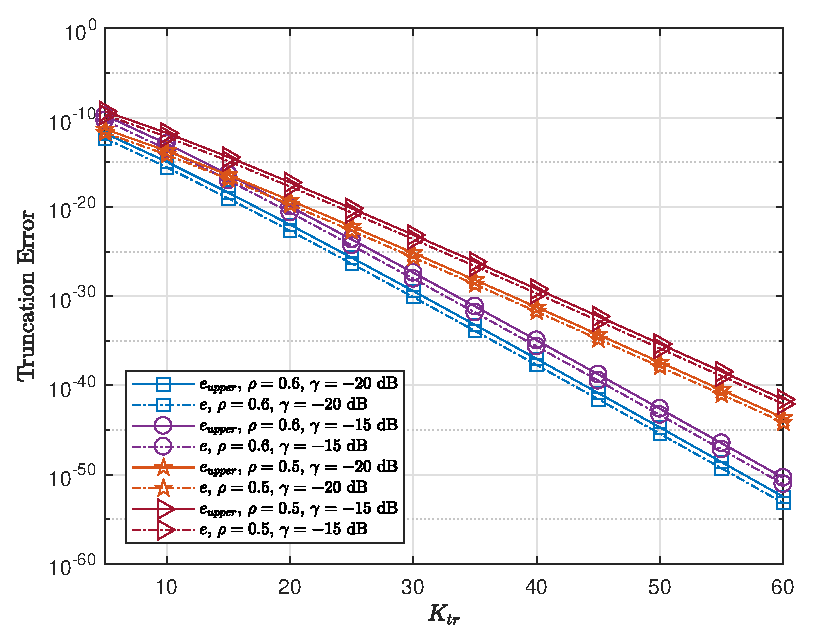
\includegraphics [width=0.45\columnwidth]{chap8_fig/rho_gamma_CDF_truncation_error.eps} 
%\vspace{-0.5cm}
\caption{Impact of $\rho$ and $\gamma$ on $e_{upper}$ for $\gamma_1 = \gamma_2 = -10$ dB and Rician $K$ factor of 7 dB.}
%\vspace{-0.2cm}
\label{fig:NOMA_bivariate_Rician_Shadowed_rho_gamma_CDF_truncation_error}
\end{figure}

Similar to Proposition \ref{NOMA_bivariate_Rician_Shadowed_proposition_df_noma_uav_j}, one obtains the asymptotic OMA diversity gain for downlink UAV-$j$ using Proposition \ref{NOMA_bivariate_Rician_Shadowed_proposition_df_oma_uav_j} as shown in the following Corollary.
%%%%%%%%%%%%%%%%%%%%%%%%%%%%%%%%%%%%%%%%%%%%%%%%%%%%%%%%%%%%%%%%%%%%%%%%%%%%%%%%%
\begin{corollary} \label{NOMA_bivariate_Rician_Shadowed_corollary_df_oma_uav_j}
At asymptotic SNR regimes, OMA achieves full diversity gain at downlink UAV-$j$, i.e., $d_{f,j}^{OMA} = 2$.
%%%%%%%%%%%%%%%%%%%%%%%%%%%%%%%%%%%%%%%%%%%%%%%%%%%%%%%%%%%%%%%%%%%%%%%%%%%%%%%%%
\end{corollary}
\begin{proof}
Corollary \ref{NOMA_bivariate_Rician_Shadowed_corollary_df_oma_uav_j} is proven in the same manner as Corollary \ref{NOMA_bivariate_Rician_Shadowed_corollary_df_noma_uav_j}. 
\end{proof}

Using Proposition \ref{NOMA_bivariate_Rician_Shadowed_proposition_df_oma_uav_j}, the finite SNR diversity gain of OMA transmissions at downlink UAV-$j$ with selection combining can now be analyzed over correlated Rician shadowed fading channels.

%OMA achieves full diversity gain due to the point-to-point nature of the links, i.e., interference-free, as shown in Corollary \ref{corollary_df_oma_uav_j}.

%%%%%%%%%%%%%%%%%%%%%%%%%%%%%%%%%%%%%%%%%%%%%%%%%%%%%%%%%%%%%%%%%%%%%%%%%%%%%%%%%%%%%%%%%%%%%%%%%%%%%%%%%%%%%%%%%%%%%%%%%%%%%%%%%%%%%%%%%
% Section 7: Numerical Results
\section{Numerical Results} \label{NOMA_bivariate_Rician_Shadowed_sec_num_res}

Numerical and simulation results pertaining to both NOMA-aided and OMA-based UCSs are presented in this section. Monte Carlo simulations were also conducted with $10^{6}$ samples, based on simulation parameters provided in Table \ref{table:NOMA_bivariate_Rician_Shadowed_sim_param} (unless otherwise stated). For the rest of the section, we present observations and discussions pertaining to the performance analysis of the NOMA-aided UCS.

\begin{table}[]
\centering
\caption{Simulation Parameters} \vspace{0.1cm}
\label{table:NOMA_bivariate_Rician_Shadowed_sim_param}
\scalebox{0.8}{\begin{tabular}{ll}
\hline
\textbf{Parameter(s)} 																					& \textbf{Value(s)}														\\  \hline \hline
Number of Downlink UAVs																					&	$N_D = 3$ \cite{wang2018modeling,tr362017}	\\
Rician $K$ Factors																							& 7\text{ dB} \cite[Table V]{matolak2017air_suburban} for $\sigma=1$	\\
Shaping Parameter																								& $m=5$	\\
Transmit Power 							 																		& $0 \leq P_t \leq 30$ (dBm)	\cite{tr362017}	\\
Path Loss Exponent 		 																					& $L = 2$\cite[Table III]{matolak2017air_suburban}, \cite{nasir2019uav} \\
Cross Correlation Coefficient 																	& $\rho = 0.5$																\\
Carrier Frequency 																							& $f_c = 2$ GHz	\cite{tr362017}								\\
Bandwidth 																											& $B_W = 10$ MHz \cite{tr362017}							\\
Transmission rate 																							& $\mathcal{R}^{OMA} = 0.1$ b/s/Hz						\\ 
Radius 																													&	$r_a = 10$ km \cite{hou2019exploiting}			\\ 
Minimum UAV Altitude																						&	$h_{min} = 0.1$ km \cite{tr362017}					\\
Altitude Separation Factor																			&	$\omega = 0.1$															\\	
Truncation Order																								& $K_{tr,1} = 30$, $K_{tr,2} = 40$						\\ \hline
\end{tabular}}
\end{table}

\subsection{Joint PDF Validation and Truncation Analysis}

Fig. \ref{fig:NOMA_bivariate_Rician_Shadowed_pdf_comp} shows a comparison between the closed-form joint PDF expression in (\ref{NOMA_bivariate_Rician_Shadowed_pwr_srs_pdf_bi_rician_shad}) and the exact expression in \cite[eq. (4)]{lopez2018bivariate}. Evidently, (\ref{NOMA_bivariate_Rician_Shadowed_pwr_srs_pdf_bi_rician_shad}) is validated as it is shown to be in very close agreement with \cite[eq. (4)]{lopez2018bivariate}. Furthermore, as $m \to \infty$, the closed-form expression in (\ref{NOMA_bivariate_Rician_Shadowed_pwr_srs_pdf_bi_rician_shad}) can be used to model a bivariate Rician fading PDF. 

The impact of the Rician $K$ factor, $m$, $\sigma$, and $\rho$ on the upper bound of the truncation error $\big(\mathcal{T}_{\epsilon,upper}\big)$ is shown in Fig. \ref{fig:NOMA_bivariate_Rician_Shadowed_truncation_error}. Likewise, the impact of $\rho$ and $\gamma$ on the upper bound of the truncation error $\big(e_{upper}\big)$ is plotted in Fig. \ref{fig:NOMA_bivariate_Rician_Shadowed_rho_gamma_CDF_truncation_error}. In particular, it is seen in Fig. \ref{fig:NOMA_bivariate_Rician_Shadowed_truncation_error} and Fig. \ref{fig:NOMA_bivariate_Rician_Shadowed_rho_gamma_CDF_truncation_error} that Lemmas \ref{NOMA_bivariate_Rician_Shadowed_lemma_te_upper} and \ref{NOMA_bivariate_Rician_Shadowed_lemma_e_upper} are validated, since $\mathcal{T}_{\epsilon} < \mathcal{T}_{\epsilon,upper}$ and $e < e_{upper}$ when $K_{tr,1}$ and $K_{tr}$ are sufficiently large. Also, Fig. \ref{fig:NOMA_bivariate_Rician_Shadowed_truncation_error} shows a small $K_{tr,1}$ leads to an insufficient number of terms to achieve convergence in the power series expressions, e.g., (\ref{NOMA_bivariate_Rician_Shadowed_pwr_srs_pdf_bi_rician_shad}), (\ref{NOMA_bivariate_Rician_Shadowed_te}), and (\ref{NOMA_bivariate_Rician_Shadowed_te_upper}). Thus, it can also be observed in Fig. \ref{fig:NOMA_bivariate_Rician_Shadowed_truncation_error} that $\mathcal{T}_{\epsilon} > \mathcal{T}_{\epsilon,upper}$ at the lower range of $K_{tr,1}$. From Fig. \ref{fig:NOMA_bivariate_Rician_Shadowed_k_factor_truncation_error}, it is seen that a larger $K_{tr,1}$ is needed to reduce $\mathcal{T}_{\epsilon,upper}$ as the Rician $K$ factor increases. It is also observed in Fig. \ref{fig:NOMA_bivariate_Rician_Shadowed_shadowing_truncation_error}, Fig. \ref{fig:NOMA_bivariate_Rician_Shadowed_sigma_truncation_error}, and Fig. \ref{fig:NOMA_bivariate_Rician_Shadowed_rho_truncation_error} that an increase in $m$, $\sigma$, and $\rho$ leads to a decrease in $\mathcal{T}_{\epsilon,upper}$. Similarly, Fig. \ref{fig:NOMA_bivariate_Rician_Shadowed_rho_gamma_CDF_truncation_error} shows that an increase in $\rho$ or decrease in $\gamma$ leads to a decrease in $e_{upper}$ Therefore, Corollaries \ref{NOMA_bivariate_Rician_Shadowed_corollary_te_upper_behavior_m_rho_sigma}, \ref{NOMA_bivariate_Rician_Shadowed_corollary_te_upper_behavior_Rician_K_factor}, and \ref{NOMA_bivariate_Rician_Shadowed_corollary_e_upper_behavior_rho_gamma} are validated.

\subsection{Outage Probability and Finite SNR Diversity Gain Analysis}
\begin{observation} 
\emph{The NOMA-aided UCS can simultaneously support more downlink UAVs on the same spectrum than an OMA-based UCS while achieving almost similar reliability.}
\end{observation}
\begin{observation} 
\emph{Smaller cross correlation corresponds to higher reliability for both NOMA and OMA transmissions.}
\end{observation}

\begin{figure} [t] 
\centering
\vspace{0.5cm}
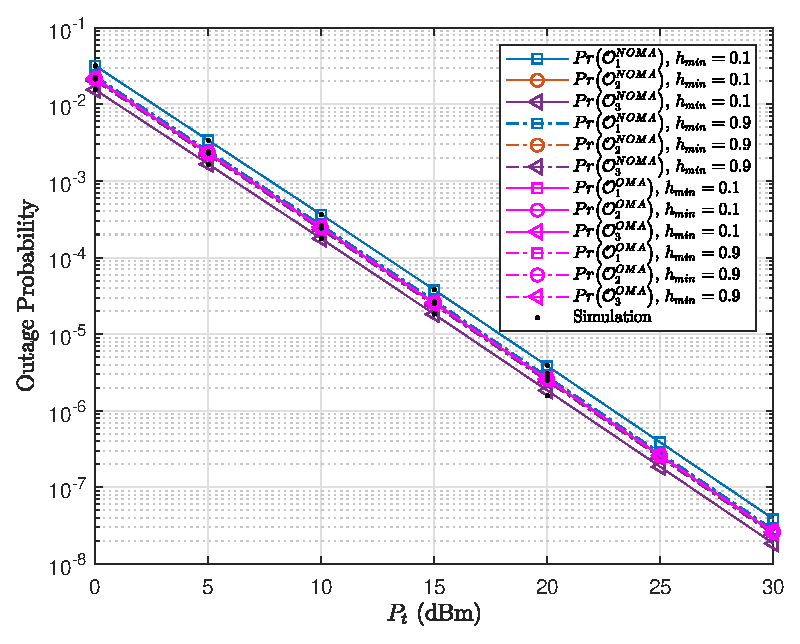
\includegraphics [width=0.45\columnwidth]{chap8_fig/outage_probability_impact_altitude.eps} 
%\vspace{-0.5cm}
\caption{Impact of minimum altitude $h_{min}$ on NOMA outage probability.}
%\vspace{-0.2cm}
\label{fig:NOMA_bivariate_Rician_Shadowed_outage_probability_impact_altitude}
\end{figure}

\begin{figure} [t] 
\centering
\vspace{0.5cm}
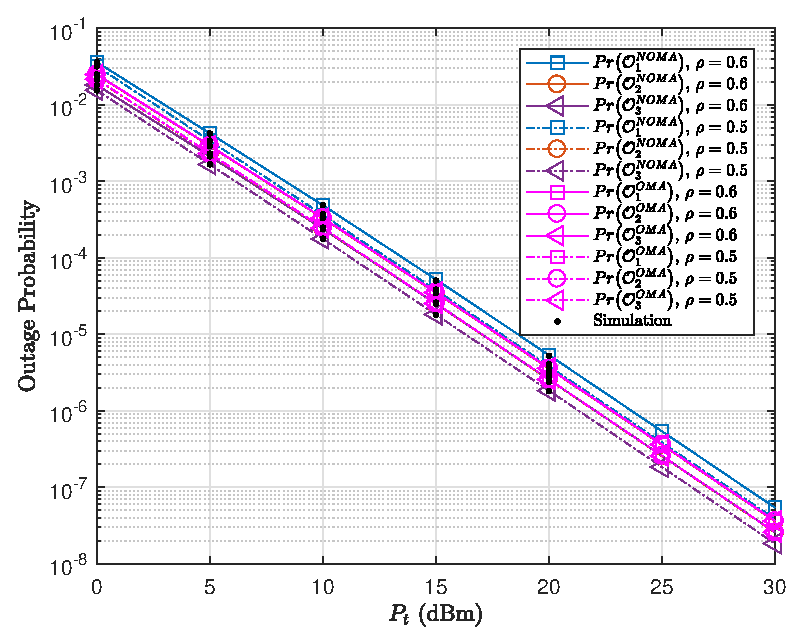
\includegraphics [width=0.45\columnwidth]{chap8_fig/outage_probability_impact_rho.eps} 
%\vspace{-0.5cm}
\caption{Impact of cross correlation coefficient $\rho$ on NOMA outage probability.}
%\vspace{-0.2cm}
\label{fig:NOMA_bivariate_Rician_Shadowed_outage_probability_impact_rho}
\end{figure}

The impact of the minimum altitude $(h_{min})$ on the NOMA outage probability of downlink UAV-$j$ $\big(Pr\big(\mathcal{O}_{j}^{NOMA}\big)\big)$ is plotted in Fig. \ref{fig:NOMA_bivariate_Rician_Shadowed_outage_probability_impact_altitude} for $1 \leq j \leq N_D$. 

It is observed that $Pr\big(\mathcal{O}_{j}^{NOMA}\big)$ is not limited by MUI, despite interference from the SOIs of other downlink UAVs. It is also seen that $Pr\big(\mathcal{O}_{j-1}^{NOMA}\big) > Pr\big(\mathcal{O}_{j}^{NOMA}\big) > Pr\big(\mathcal{O}_{j+1}^{NOMA}\big)$ at low $h_{min}$. Such an occurrence is due to the power allocation factor $(a_j)$, which is larger for downlink UAVs operating at higher altitudes $(h_j)$. Specifically, when $h_{min}$ is low, the difference between $a_j$ and $a_{j+1}$ is larger, leading to lower NOMA outage probability for downlink UAVs at higher altitudes. As $h_{min}$ is increased, the difference between $a_j$ and $a_{j+1}$ diminishes due to the altitude separation factor $(\omega)$. Thus, the downlink UAVs exhibit very similar NOMA outage probabilities for $h_{min} = 0.9$. When compared against the OMA-based UCS, it is evident that the NOMA-aided UCS achieve similar outage probability particularly at high $h_{min}$. Therefore, the NOMA-aided UCS is able to achieve similar reliability to an OMA-based UCS while simultaneously \textcolor{black}{supporting} a greater number of downlink UAVs. 

The impact of the cross correlation coefficient $(\rho)$ on the NOMA outage probability of downlink UAV-$j$, i.e., $Pr\big(\mathcal{O}_{j}^{NOMA}\big)$, is plotted in Fig. \ref{fig:NOMA_bivariate_Rician_Shadowed_outage_probability_impact_rho} for $1 \leq j \leq N_D$. It is seen that an increase in $\rho$ corresponds to an increase in $Pr\big(\mathcal{O}_{j}^{NOMA}\big)$ and $Pr\big(\mathcal{O}_{j}^{OMA}\big)$. Such a behavior is due to the decrease in diversity gain, i.e., $d_{f,j}^{NOMA}$ and $d_{f,j}^{OMA}$, as cross correlation $(\rho)$ increases \cite{lopez2018bivariate}. 

\begin{figure} [] 
\centering
\vspace{0.5cm}
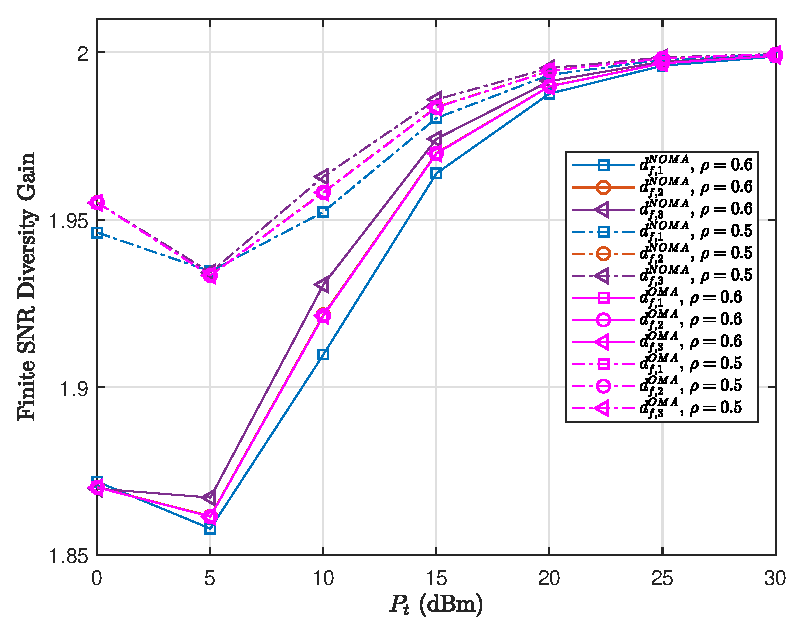
\includegraphics [width=0.45\columnwidth]{chap8_fig/finite_snr_diversity_gain_impact_rho.eps} 
%\vspace{-0.5cm}
\caption{Impact of cross correlation coefficient $\rho$ on NOMA finite SNR diversity gain.}
%\vspace{-0.2cm}
\label{fig:NOMA_bivariate_Rician_Shadowed_finite_snr_diversity_gain_impact_rho}
\end{figure}

A clearer picture of the outage probability decay behavior is seen in Fig. \ref{fig:NOMA_bivariate_Rician_Shadowed_finite_snr_diversity_gain_impact_rho}, where $d_{f,j}^{NOMA}$ and $d_{f,j}^{OMA}$ is plotted for $1 \leq j \leq N_D$. Specifically, similar trends are also observed in Fig. \ref{fig:NOMA_bivariate_Rician_Shadowed_finite_snr_diversity_gain_impact_rho} at low $P_t$ regimes, with both NOMA and OMA transmissions experiencing lower $d_{f,j}^{NOMA}$ and $d_{f,j}^{OMA}$, respectively, as $\rho$ is increased. However, at high $P_t$ regimes, it is observed that the impact of $\rho$ diminishes since both $d_{f,j}^{NOMA} \to 2$ and $d_{f,j}^{OMA} \to 2$ as $P_t$ increases. Such an observation is due to the fact that $\rho$ only affects the coding gain of selection combining techniques \cite{el2015mimo}. In particular, the coding gain of both NOMA and OMA transmissions increases as $P_t$ increases at low $P_t$ regimes. As a result, a lower $d_{f,j}^{NOMA}$ and $d_{f,j}^{OMA}$ is experienced when $\rho$ is increased. However, at high $P_t$ regimes, the increase in the coding gain becomes negligible. Hence, $d_{f,j}^{NOMA} = d_{f,j}^{OMA} = 2$ for $\rho \in\{0.5, 0.6\}$, which validate Corollaries \ref{NOMA_bivariate_Rician_Shadowed_corollary_df_noma_uav_j} and \ref{NOMA_bivariate_Rician_Shadowed_corollary_df_oma_uav_j}. Therefore, it is demonstrated that a low cross correlation is required in order to achieve a lower outage probability for the NOMA-aided UCS. Additionally, the coding gain of selection combining for both NOMA and OMA transmissions becomes stagnant at high $P_t$ regimes.  



%The impact of the cross correlation coefficient $(\rho)$ on the NOMA outage probability and finite SNR diversity gain $d_{f,j}^{NOMA}$ of downlink UAV-$j$ is respectively plotted in Fig. \ref{fig:outage_probability_impact_rho} and Fig. \ref{fig:finite_snr_diversity_gain_impact_rho} for $1 \leq j \leq N_D$. 





%%%%%%%%%%%%%%%%%%%%%%%%%%%%%%%%%%%%%%%%%%%%%%%%%%%%%%%%%%%%%%%%%%%%%%%%%%%%%%%%%%%%%%%%%%%%%%%%%%%%%%%%%%%%%%%%%%%%%%%%%%%%%%%%%%%%%%%%%
% Section 8: Conclusion
\section{Chapter Summary} \label{NOMA_bivariate_Rician_Shadowed_sec_conclusion}
To address spectrum scarcity in UAV communications, a NOMA-aided UCS with dual-antenna downlink UAVs employing selection combining is investigated in this chapter. Through new closed-form expressions for the joint PDF and joint CDF, new expressions pertaining to the outage probability and finite SNR diversity gain of the NOMA-aided UCS are presented. It is shown that more downlink UAVs can be supported on the same spectrum with the NOMA-aided UCS, with an outage probability that is similar to OMA-based UCSs. Furthermore, the effect of cross correlation is analyzed, where it is shown that lower correlation leads to lower outage probability in the NOMA-aided UCS. Also, it is demonstrated that correlation only reduces the diversity gain of NOMA-aided and OMA-based UCSs at low SNR regimes. Therefore, NOMA-aided UCSs are an attractive alternative over OMA-based schemes in future wireless systems.




